\documentclass[12pt]{article}

% MLA format
\usepackage[letterpaper]{geometry}
\usepackage{times}
\geometry{top=1.0in, bottom=1.0in, left=1.0in, right=1.0in}
\usepackage{fancyhdr}
\pagestyle{fancy}
\lhead{} 
\chead{} 
\rhead{Simmons \thepage} 
\lfoot{} 
\cfoot{} 
\rfoot{}
\renewcommand{\headrulewidth}{0pt} 
\renewcommand{\footrulewidth}{0pt} 

\usepackage{mdwlist}
\usepackage{enumitem}
\setlist{  
  listparindent=\parindent,
  parsep=0pt,
}
\title{Homework 8}
\author{Mark Simmons}
\date{April 17, 2020}


% Typing in IPA
%\usepackage{tipa}

% Sentence trees
\usepackage{tikz}
\usepackage{tikz-qtree}
\usepackage{lscape}
\usepackage{graphicx}
\usepackage{pstricks}
\usepackage{tree-dvips}
\tikzset{level distance=30pt,
    sibling distance=6pt,
    every tree node/.style={align=center},
    }

\begin{document}

\maketitle



\begin{enumerate}[label=\textbf{\arabic*.}]

\item \textbf{Technical}

	\begin{enumerate}[label=(\alph*)]

	% He always ate carrots
	\item Deep Structure\\
	\bigskip
	\leavevmode\vadjust{\vspace{-\baselineskip}}\newline
	%\begin{landscape}
	\noindent{\begin{tikzpicture}
	{\small \Tree
	[.CP {}
	[.C' C\\$\emptyset$
	[.TP {}
	[.T' T\\-ed
		[.VP [.DP \edge[roof]; {He} ]
		[.V' [.AdvP \edge[roof]; {always} ]
			[.V' V\\eat
				[.DP \edge[roof]; {carrots} ]
			]%V'
		]%V'
		]%VP
	]%T'
	]%TP
	]%C'
	]%CP
	}
	\end{tikzpicture}}

	\pagebreak

	\noindent Surface Structure\\
	\bigskip

	\noindent{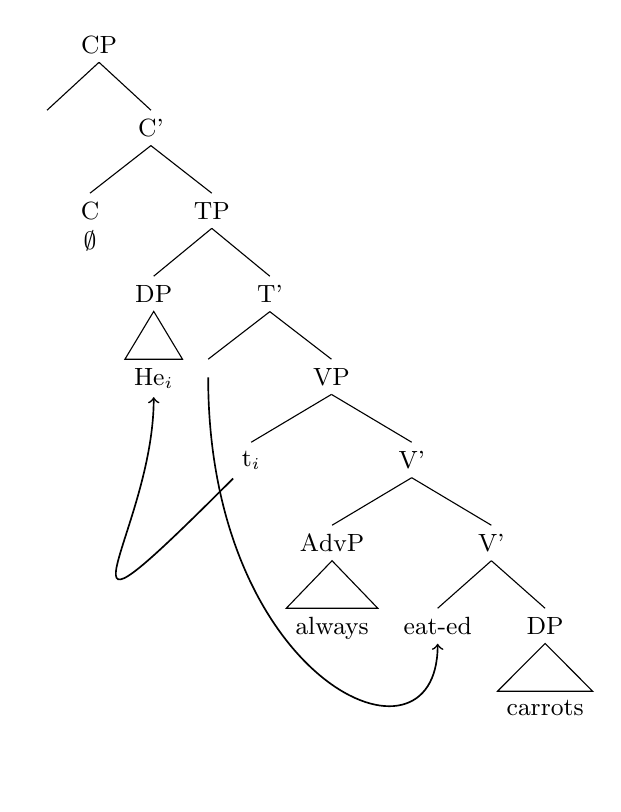
\begin{tikzpicture}
	\tikzset{every tree node/.style={align=center,anchor=north}}
	{\small \Tree
	[.CP {}
	[.C' C\\$\emptyset$
	[.TP [.DP \edge[roof]; \node(a){He$_{i}$}; ]
	[.T' \node(c){}; 
		[.VP \node(b){t$_{i}$};
		[.V' [.AdvP \edge[roof]; {always} ]
			[.V' \node(d){eat-ed};
				[.DP \edge[roof]; {carrots} ]
			]%V'
		]%V'
		]%VP
	]%T'
	]%TP
	]%C'
	]%CP
	\draw[semithick,->] (b)..controls +(south west:4) and +(south:2)..(a);
	\draw[semithick,->] (c)..controls +(south:4) and +(south:2)..(d);
	}
	\end{tikzpicture}}

	% He has always eaten carrots
	\item Deep Structure\\
	\bigskip
	\leavevmode\vadjust{\vspace{-\baselineskip}}\newline
	%\begin{landscape}
	\noindent{\begin{tikzpicture}
	{\small \Tree
	[.CP {}
	[.C' C\\$\emptyset$
	[.TP {}
	[.T' T\\-s
		[.VP [.DP \edge[roof]; {He} ]
		[.V' [.AdvP \edge[roof]; {always} ]
			[.V' V\\have
				[.V' V\\eaten
				[.DP \edge[roof]; {carrots} ]
				]%V'
			]%V'
		]%V'
		]%VP
	]%T'
	]%TP
	]%C'
	]%CP	
	}
	\end{tikzpicture}}


	\pagebreak

	\noindent Surface Structure\\
	\bigskip

	\noindent{\begin{tikzpicture}
	\tikzset{every tree node/.style={align=center,anchor=north}}
	{\small \Tree
	[.CP {}
	[.C' C\\$\emptyset$
	[.TP [.DP \edge[roof]; \node(a){He$_{i}$}; ]
	[.T' \node(c){T\\has$_{j}$}; 
		[.VP \node(b){t$_{i}$};
		[.V' [.AdvP \edge[roof]; {always} ]
			[.V' \node(d){t$_{j}$};
				[.V' V\\eaten
				[.DP \edge[roof]; {carrots} ]
				]%V'
			]%V'
		]%V'
		]%VP
	]%T'
	]%TP
	]%C'
	]%CP
	\draw[semithick,->] (b)..controls +(south west:4) and +(south:2)..(a);
	\draw[semithick,->] (d)..controls +(south:4) and +(south:2)..(c);
	}
	\end{tikzpicture}}

	\pagebreak

	% He does not love carrots
	\item Deep Structure\\
	\bigskip
	\leavevmode\vadjust{\vspace{-\baselineskip}}\newline
	%\begin{landscape}
	\noindent{\begin{tikzpicture}
	{\small \Tree
	[.CP {}
	[.C' C\\$\emptyset$
	[.TP {}
	[.T' T\\-s
		[.NegP [.AdvP \edge[roof]; {not} ]
		[.Neg' Neg\\-$\emptyset$
		[.VP [.DP \edge[roof]; {He} ]
			[.V' V\\love
				[.DP \edge[roof]; {carrots.} ]
			]%V'
		]%VP
		]%Neg'
		]%NegP
	]%T'
	]%TP
	]%C'
	]%CP	
	}
	\end{tikzpicture}}


	\pagebreak

	\noindent Surface Structure\\
	\bigskip

	\noindent{\begin{tikzpicture}
	\tikzset{every tree node/.style={align=center,anchor=north}}
	{\small \Tree
	[.CP {}
	[.C' C\\$\emptyset$
	[.TP [.DP \edge[roof]; \node(b){He$_{i}$}; ]
	[.T' \node[draw,circle]{T\\does};
		[.NegP [.AdvP \edge[roof]; {not} ]
		[.Neg' \node(c){Neg};
		[.VP \node(a){t$_{i}$};
			[.V' \node(d){V\\love$-\emptyset$};
				[.DP \edge[roof]; {carrots.} ]
			]%V'
		]%VP
		]%Neg'
		]%NegP
	]%T'
	]%TP
	]%C'
	]%CP	
	}
	\draw[dashed,->] (a)..controls +(south:4) and +(south:4)..(b);
	%\draw[semithick,->] (d)..controls +(south:4) and +(south:2)..(c);
	\draw[semithick,->] (c)..controls +(south:4) and +(south:2)..(d);
	\end{tikzpicture}}

	\pagebreak

	% Have you always been eating carrots?
	\item Deep Structure\\
	\bigskip
	\leavevmode\vadjust{\vspace{-\baselineskip}}\newline
	%\begin{landscape}
	\noindent{\begin{tikzpicture}
	{\small \Tree
	[.CP {}
	[.C' C\\-$\emptyset_{[+Q]}$
	[.TP {}
	[.T' T\\-$\emptyset_{[+present]}$
		[.VP [.DP \edge[roof]; {you} ]
		[.V' [.AdvP \edge[roof]; {always} ]
			[.V' V\\Have
				[.V' V\\been
					[.V' V\\eating
					[.DP \edge[roof]; {carrots?} ]
					]%V'
				]%V'
			]%V'
		]%V'
		]%VP
	]%T'
	]%TP
	]%C'
	]%CP	
	}
	\end{tikzpicture}}


	\pagebreak

	\noindent Surface Structure\\
	\bigskip

	\noindent{\begin{tikzpicture}
	\tikzset{every tree node/.style={align=center,anchor=north}}
	{\small \Tree
	[.CP {}
	[.C' \node(e){C\\Have-$\emptyset_{j}$}; 
	[.TP [.DP \edge[roof]; \node(a){you$_{i}$}; ]
	[.T' \node(c){T\\t$_{j}$}; 
		[.VP \node(b){t$_{i}$};
		[.V' [.AdvP \edge[roof]; {always} ]
			[.V' \node(d){t$_{j}$};
				[.V' V\\been
				[.V' V\\eating
				[.DP \edge[roof]; {carrots} ]
				]%V'
				]%V'
			]%V'
		]%V'
		]%VP
	]%T'
	]%TP
	]%C'
	]%CP
	\draw[dashed,->] (b)..controls +(south:4) and +(south:4)..(a);
	\draw[semithick,->] (d)..controls +(south:4) and +(south:2)..(c);
	\draw[semithick,->] (c)..controls +(south:4) and +(south:2)..(e);
	}
	\end{tikzpicture}}

	\pagebreak

	% Martha should think John does not hate phonology.
	\item Deep Structure\\
	\bigskip
	\leavevmode\vadjust{\vspace{-\baselineskip}}\newline
	%\begin{landscape}
	\noindent{\begin{tikzpicture}
	{\small \Tree
	[.CP {}
	[.C' C\\$\emptyset$
	[.TP {}
	[.T' T\\should
	[.VP [.DP \edge[roof]; Martha ]
	[.V' V\\think
		[.CP {}
		[.C' C\\$\emptyset$
		[.TP {}
		[.T' T\\-s
		[.NegP [.AdvP \edge[roof]; not ]
		[.Neg' Neg\\-$\emptyset$
		[.VP [.DP \edge[roof]; John ]
		[.V' V\\hate [.DP \edge[roof]; phonology. ]
		]%V'
		]%VP
		]%Neg'
		]%NegP
		]%T'
		]%TP
		]%C'
		]%CP
	]%V'
	]%VP
	]%T'
	]%TP
	]%C'
	]%CP	
	}
	\end{tikzpicture}}


	\pagebreak

	\noindent Surface Structure\\
	\bigskip

	\noindent{\begin{tikzpicture}
	\tikzset{every tree node/.style={align=center,anchor=north}}
	{\small \Tree
	[.CP {}
	[.C' C\\$\emptyset$
	[.TP [.DP \edge[roof]; \node(upperSub){Martha$_{i}$}; ]
	[.T' T\\should
	[.VP \node(upperTrace){t$_{i}$};
	[.V' V\\think
		[.CP {}
		[.C' C\\$\emptyset$
		[.TP [.DP \edge[roof]; \node(lowerSub){John$_{j}$}; ]
		[.T' \node[draw,circle]{T\\does};
		[.NegP [.AdvP \edge[roof]; not ]
		[.Neg' \node(negAffix){Neg};
		[.VP \node(lowerTrace){t$_{j}$};
		[.V' \node(negV){V\\hate-$\emptyset$}; [.DP \edge[roof]; phonology. ]
		]%V'
		]%VP
		]%Neg'
		]%NegP
		]%T'
		]%TP
		]%C'
		]%CP
	]%V'
	]%VP
	]%T'
	]%TP
	]%C'
	]%CP
	%\draw[dashed,->] (b)..controls +(south:4) and +(south:4)..(a);
	%\draw[semithick,->] (d)..controls +(south:4) and +(south:2)..(c);
	%\draw[semithick,->] (c)..controls +(south:4) and +(south:2)..(e);
	\draw[semithick, ->] (upperTrace)..controls +(south:2) and +(south:3)..(upperSub);
	\draw[semithick, ->] (lowerTrace)..controls +(south:2) and +(south:4)..(lowerSub);
	\draw[dashed, ->] (negAffix)..controls +(south:4) and +(south:1)..(negV);


	}
	\end{tikzpicture}}

	\pagebreak

	% Les enfants n'ont pas travaillé
	\item Deep Structure\\
	\bigskip
	\leavevmode\vadjust{\vspace{-\baselineskip}}\newline
	%\begin{landscape}
	\noindent{\begin{tikzpicture}
	{\small \Tree
	[.CP {}
	[.C' C\\$\emptyset$
	[.TP {}
	[.T' T\\-ent
		[.NegP [.AdvP \edge[roof]; pas ]
		[.Neg' Neg\\ne=
		[.VP [.DP \edge[roof]; {Les enfants} ]
		[.V' V\\avoir
			[.V' V\\travaillé {} ]
		]%V'
		]%VP
		]%Neg'
		]%NegP
	]%VP
	]%T'
	]%TP
	]%C'
	]%CP	
	}
	\end{tikzpicture}}


	\pagebreak

	\noindent Surface Structure\\
	\bigskip

	\noindent{\begin{tikzpicture}
	\tikzset{every tree node/.style={align=center,anchor=north}}
	{\small \Tree
	[.CP {}
	[.C' C\\$\emptyset$
	[.TP [.DP \edge[roof]; \node(sub){Les enfants}; ]
	[.T' \node(auxT){T\\n'ont};
		[.NegP [.AdvP \edge[roof]; pas ]
		[.Neg' \node(negAffix){Neg};
		[.VP \node(trace){t$_{i}$};
		[.V' \node(auxTrace){t$_{i}$};
			[.V' V\\travaillé {}
			]%V'
		]%V'
		]%VP
		]%Neg'
		]%NegP
	]%VP
	]%T'
	]%TP
	]%C'
	]%CP	
	\draw[semithick, ->] (trace)..controls +(south:2) and +(south:6)..(sub);
	%\draw[semithick, ->] (lowerTrace)..controls +(south:2) and +(south:4)..(lowerSub);
	\draw[dashed, ->] (negAffix)..controls +(south:5) and +(south:1)..(auxTrace);
	\draw[dotted, ->] (auxTrace)..controls +(south:1) and +(south:5)..(auxT);

	}
	\end{tikzpicture}}

	\pagebreak

	% Les enfants ne travaillent pas.
	\item Deep Structure\\
	\bigskip
	\leavevmode\vadjust{\vspace{-\baselineskip}}\newline
	%\begin{landscape}
	\noindent{\begin{tikzpicture}
	{\small \Tree
	[.CP {}
	[.C' C\\$\emptyset$
	[.TP {}
	[.T' T\\-ent
		[.NegP [.AdvP \edge[roof]; pas ]
		[.Neg' Neg\\ne=
		[.VP [.DP \edge[roof]; {Les enfants} ]
		[.V' V\\travailler {}
		]%V'
		]%VP
		]%Neg'
		]%NegP
	]%VP
	]%T'
	]%TP
	]%C'
	]%CP	
	}
	\end{tikzpicture}}


	\pagebreak

	\noindent Surface Structure\\
	\bigskip

	\noindent{\begin{tikzpicture}
	\tikzset{every tree node/.style={align=center,anchor=north}}
	{\small \Tree
	[.CP {}
	[.C' C\\$\emptyset$
	[.TP [.DP \edge[roof]; \node(sub){Les enfants$_{i}$}; ]
	[.T' \node(vT){T\\ne travaillent$_{j}$};
		[.NegP [.AdvP \edge[roof]; pas ]
		[.Neg' \node(negAffix){Neg};
		[.VP \node(subTrace){t$_{i}$};
		[.V' \node(vTrace){t$_{j}$}; {}
		]%V'
		]%VP
		]%Neg'
		]%NegP
	]%VP
	]%T'
	]%TP
	]%C'
	]%CP	
	\draw[semithick, ->] (subTrace)..controls +(south:2) and +(south:6)..(sub);
	%\draw[semithick, ->] (lowerTrace)..controls +(south:2) and +(south:4)..(lowerSub);
	\draw[dashed, ->] (negAffix)..controls +(south:5) and +(south:1)..(vTrace);
	\draw[dotted, ->] (vTrace)..controls +(south:1) and +(south:5)..(vT);

	}
	\end{tikzpicture}}

	\end{enumerate}

\item \textbf{Short Answer}

	\begin{enumerate}[label=(\alph*)]
	\item \textbf{German:} In the presence of auxiliaries, e.g. \emph{sollen} and \emph{sein}, verbs appear at the
	end of the clause (v. 2b,d), whereas the auxiliary appears closer to the beginning of the clause. In (2a,c)
	no auxiliary is present and the verb (\emph{sprechen} and \emph{sitzt} respectively) appears near the 
	beginning of the clause. Furthermore, the negative particle intervenes between the verb \emph{sitzt} and
	the verb complement \emph{auf disem Tish} in (2c), suggesting that the verb has moved from outside the VP.
	Thus, German appears to have V $\rightarrow$ T movement.

	\item \textbf{Indonesian:} (3a,b) show that the modal auxiliary \emph{boleh} precedes the verb \emph{masuk}
	in a declarative clause, and appears clause-initially in an interrogative clause. In (3d), the verb
	\emph{membeli} fronts in an interrogative clause, suggesting that V can move to T (which then moves to C),
	thus Indonesian appears to have V $\rightarrow$ T movement.

	\item \textbf{Haitian:} The past auxiliary \emph{te} occurs before the adverb \emph{deja}. The verb
	\emph{pase} occurs after the adverb \emph{deja} and before the object \emph{rad yo} whether \emph{te}
	is present or not in the sentence. Interjecting the adverb between the verb and the object results in 
	an ungrammatical sentence, as shown in (4c,d). Thus, V does not appear to move to T, suggesting that
	Haitian Creole features T $\rightarrow$ V lowering.

	\textbf{Bonus:} If we assume that \emph{pa} behaves similar to \emph{not} in English and \emph{pas} in
	French, then we would expect it to follow T and precede V. \emph{renmen} is of category V, and (5a) shows
	that NEG precedes it. Furthermore, (5b) shows that \emph{renmen} does not raise to T, since placing NEG
	after it results in an ungrammatical sentence.
	\end{enumerate}

\item \textbf{Argumentation}
	
	German exhibits V2 word order, a phenomenon where the topic phrase of a CP occurs as the first element,
	followed by the finite verb.

	\begin{enumerate}[label=(\arabic*)]
		\item
		\begin{enumerate}[label=\alph*.]
		\item Die Kinder \emph{haben} diesen Film gesehen.\\
		`The children have seen this film.'
		\item Diesen Film \emph{haben} die Kinder gesehen.\\
		`The children have seen this film.'
		\end{enumerate}
	\suspend{enumerate}

	In complement clauses introduced by \emph{daß}, however, the finite verb does not appear following
	the topic phrase, but rather at the very end of the sentence.

	\resume{enumerate}[{[label=(\arabic*)]}]
		\item
		\begin{enumerate}[label=\alph*.]
		\item Er sagt [ daß die Kinder diesen Film gesehen haben ].\\
		`He said that the children have seen this film.'
		\item *Er sagt [ daß die Kinder haben diesen Film gesehen ].
		\end{enumerate}
	\suspend{enumerate}

	In X-Bar theory, phrase heads that ``jump around'' between various places in a sentence can
	be explained by rules of movement that operate on output from the deep structure (DS) of a
	sentence, being reflected in the surface structure (SS). In French, for example, V arguments
	move to T position when T is occupied by a stranded affix. In this paper. I will argue that
	V2 word order as observed in German is best explained as a movement process that occurs because of a stranted affix
	in C position that causes the topic DP as well as the T to front.

	If we assume that subject moves from specifier to VP to specifier to TP, and that V raises
	to T when T is occupied by a stranded affix, we can generate a tree for the inner clause
	of (2a) without any further movement rules.

	\pagebreak

	\resume{enumerate}[{[label=(\arabic*)]}]
	\item
	\leavevmode\vadjust{\vspace{-\baselineskip}}\newline
	\noindent{\begin{tikzpicture}
	\tikzset{every tree node/.style={align=center,anchor=north}}
	{\small \Tree
	[.CP {}
	[.C' C\\daß
	[.TP [.DP \edge[roof]; \node(sub){die Kinder$_{i}$}; ]
	[.T'
	[.VP \node(subTrace){t$_{i}$};
	[.V'
		[.V' [.DP \edge[roof]; {diesen Film} ]
		V\\gesehen
		]
		\node(vTrace){t$_{j}$};
	]%V'
	]%VP
	\node(vT){haben}; ]%T'
	]%TP
	]%C'
	]%CP	
	\draw[semithick, ->] (subTrace)..controls +(south:2) and +(south:6)..(sub);
	\draw[dashed, ->] (vTrace)..controls +(south:1) and +(south:5)..(vT);

	}
	\end{tikzpicture}}
	\suspend{enumerate}

	However, we cannot generate the outer clause with these same rules. As observed above,
	our model currently predicts that all V and T arguments occur after the complement of VP,
	which would generate the ungrammatical sentence
	\emph{*Er [ daß die Kinder haben diesen Film gesehen ] sagt. } We need another rule to
	explain why T precedes the complement of VP rather than following it.

	As noted above, T is only attested to occur clause-finally when \emph{daß} is in C position. The same
	sentence as (2a) without an overt C introducing the embedded clause features T in clause-initial position.

	\resume{enumerate}[{[label=(\arabic*)]}]
	\item \%Er sagt [ die Kinder haben diesen Film gesehen ].\\
	`He said that the children have seen this film.'
	\suspend{enumerate}

	Here, we see T occuring immediately before the complement of \emph{gesehen} (i.e. the DP \emph{diesen Film}), same as in (1a). It would appear
	T has fronted, but it is not clear to what position. Since it is interposed between the subject DP \emph{die
	Kinder} and the V \emph{gesehen}, it is possible that it is moved to the specifier position of VP, which is
	between the same two arguments in (3). However, it is important to note that specifier-VP in (3) is not empty,
	rather it is occupied by a trace from the subject. Furthermore, it is worth noting that T is only attested
	in initial position when C seems to be empty. I thus propose that T raises to the C position when C is not
	occupied by an overt lexeme. This is because in the absence of an overt lexeme like \emph{daß}, C is occupied
	by a null affix. T then raises to satisfy the Stranded Affix Filter.

	This leaves the question of why T is preceded by the subject DP. In (3), nothing precedes C \emph{daß} except for an
	empty specifier position. Thus, if we only proposed that T raises to C, we would expect T to appear at the
	beginning of the sentence, with nothing preceding it. This can be resolved by applying a second movement rule,
	which moves the subject DP to specifier of CP position, correctly predicting the following tree for (2a):

	\resume{enumerate}[{[label=(\arabic*)]}]
	\item
	\leavevmode\vadjust{\vspace{-\baselineskip}}\newline
	\noindent{\begin{tikzpicture}
	\tikzset{every tree node/.style={align=center,anchor=north}}
	{\small \Tree
	[.CP [.DP \edge[roof]; \node(specCP){Er$_{i}$}; ]
	[.C' \node(vC){C\\sagt-$\emptyset_{[+Topic]j}$};
	[.TP \node(specTP){t$_{i}$};
	[.T' \node(traceT){t$_{j}$};
	[.VP \node(subTraceUpper){t$_{i}$};
	[.V' \node(vTraceUpper){t$_{j}$};
		[.CP {}
		[.C' C\\daß
		[.TP [.DP \edge[roof]; \node(sub){die Kinder$_{k}$}; ]
		[.T'
		[.VP \node(subTrace){t$_{k}$};
		[.V'
		[.V' [.DP \edge[roof]; {diesen Film} ]
		V\\gesehen
		]
		\node(vTrace){t$_{l}$};
		]%V'
		]%VP
		\node(vT){haben$_{l}$};
		]%T'
		]%TP
		]%C'
		]%CP
	]%V'
	]%VP
	]%T'
	]%TP
	]%C'	
	]%CP
	\draw[semithick, ->] (subTrace)..controls +(south:2) and +(south:6)..(sub);
	\draw[dashed, ->] (vTrace)..controls +(south:1) and +(south:5)..(vT);
	\draw[dashed, ->] (vTraceUpper)..controls +(south:1) and +(south:5)..(traceT);
	\draw[dashed, ->] (traceT)..controls +(south:1) and +(south:5)..(vC);
	\draw[semithick, ->] (subTraceUpper)..controls +(south:2) and +(south:3)..(specTP);
	\draw[semithick, ->] (specTP)..controls +(south:2) and +(south:3)..(specCP);

	}
	\end{tikzpicture}}
	\suspend{enumerate}

	We can explain why the subject DP raises if we posit that it bears an uninterpetable feature [+TopicU]. This
	then requires the DP to migrate to specifier of CP position in order to check this feature. However, the fronted
	DP is not always the subject of the sentence, as demonstrated below.

	\resume{enumerate}[{[label=(\arabic*)]}]
	\item Diesen Film \emph{haben} die Kinder gesehen.\\
	`The children have seen this film.'
	\suspend{enumerate}

	And this is why I propose the topic feature. In (1a) and (2a), the topic of the sentence is the subject DP, but initially
	(2a) it is the object. Thus in (2a) the object DP migrates to specifier of CP position, leaving the subject as the specifier
	of TP, which follows the verb in C position, generating the correct surface structure for the sentence. Note that, since
	[+Topic] is a pragmatic rather than morphological feature, my theory permits that phrase types other than DP can be fronted
	in the same manner, but no such example is attested in the data concerned.

	Thus, we can explain the V2 tendency in German by positing a phonologically null affix that occupies C position
	whenever no lexical C appears present. This affix causes the T to raise to C position in order to satisfy the Stranded
	Affix Filter, and then requires the topic phrase to front in order for its [+TopicU] feature to be checked.

\end{enumerate}
\end{document}
